\item[(e)]
\section{FIR Filter Design with Rectangular Window}

\subsection*{Problem Statement}
Design an FIR filter of order \( N = 20 \) with a rectangular window with a corner radian frequency \( \Omega_0 \). Plot its frequency response and the tolerance scheme in one plot. To this end, complete the provided file `dsp_5_4.m`.

\subsection*{Theoretical Background}
The rectangular window is a simple window function that can be used to truncate the ideal impulse response to a finite length. The frequency response of the resulting FIR filter can then be analyzed and compared with the specified tolerance scheme.

\subsection*{Mathematical Derivation}
The ideal impulse response is given by:
\[ h_{\text{ideal}}[n] = 0.37 \, \text{sinc}(0.37n) \]

To design an FIR filter of order \( N = 20 \) with a rectangular window:
\begin{itemize}
    \item Generate the ideal impulse response \( h_{\text{ideal}}[n] \) for \( n = -10 \) to \( 10 \) (centered around zero).
    \item Apply the rectangular window, which in this case does not change the values of \( h_{\text{ideal}}[n] \) because the window is entirely non-zero over the range.
    \item The resulting windowed and shifted impulse response is the FIR filter coefficients.
\end{itemize}

\subsection*{Implementation and Results}
The frequency response of the designed FIR filter is computed and plotted using Python. The plot below illustrates the frequency response along with the specified tolerance scheme.

\begin{figure}[h]
    \centering
    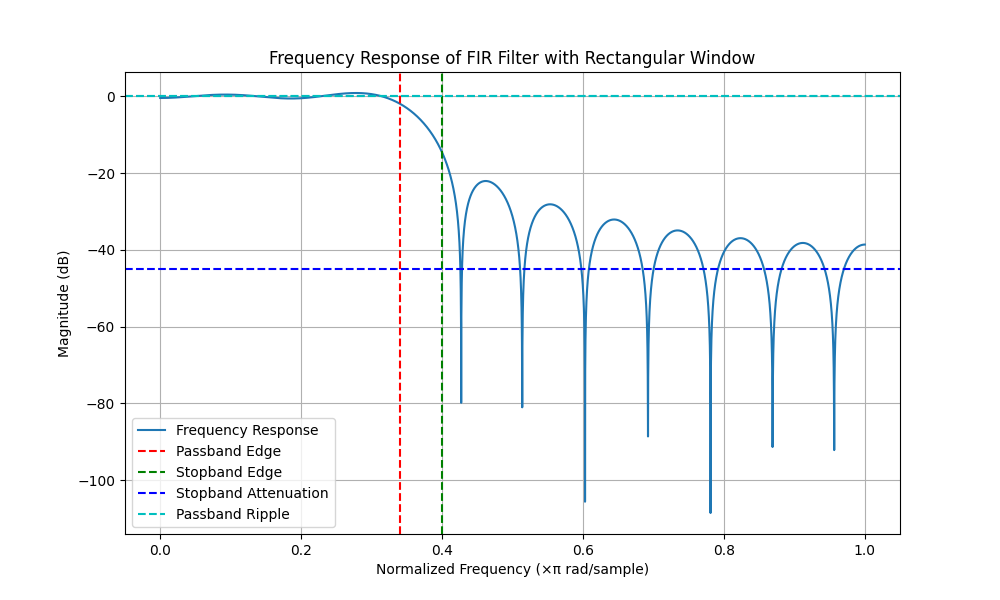
\includegraphics[width=0.8\textwidth]{fig/ex4_e_frequency_response.png}
    \caption{Frequency Response of FIR Filter with Rectangular Window}
    \label{fig:ex4_e_frequency_response}
\end{figure}

\subsection*{Conclusion}
The frequency response plot shows the performance of the FIR filter designed with a rectangular window of order \( N = 20 \). The tolerance scheme is also illustrated for comparison.
